\subsection{Slučaj upotrebe: Izmena scenarija}

\subsubsection*{Kratak opis}

Scenarista menja postojeći scenario i čuva izmene kao novu verziju, koju šalje
reditelju na odobravanje. Reditelj odobrava verziju ili je vraća na doradu.
Scenarista može da pregleda istoriju verzija i da se vrati na neku od
prethodnih.

\subsubsection*{Akteri}
\begin{itemize}
    \item \textbf{Scenarista} -- menja scenario i šalje novu verziju na odobravanje.
    \item \textbf{Reditelj} -- pregleda poslatu verziju i odobrava je ili vraća na doradu.
\end{itemize}

\subsubsection*{Preduslovi}
\begin{itemize}
    \item Scenarista je prijavljen na sistem i angažovan na projektu.
    \item Reditelj je angažovan na projektu.
    \item Za projekat je kreiran scenario (slučaj upotrebe ,,Kreiranje scenarija'').
\end{itemize}

\subsubsection*{Postuslovi}
\begin{itemize}
    \item Izmene su sačuvane kao nova verzija scenarija, a prethodne verzije ostaju nepromenjene.
    \item Reditelj je doneo odluku o poslatoj verziji, a scenarista je o njoj obavešten.
\end{itemize}

\subsubsection*{Osnovni tok}
\begin{enumerate}
    \item Scenarista bira projekat i opciju ,,Izmeni scenario''.
    \item Sistem prikazuje najnoviju verziju scenarija i istoriju verzija.
    \item Scenarista menja podatke scenarija i/ili scene (dodaje ih, menja i briše).
    \item Scenarista bira opciju ,,Sačuvaj kao novu verziju'' i unosi napomenu o izmenama.
    \item Sistem proverava podatke i čuva izmene kao novu verziju sa sledećim rednim brojem i statusom ,,U izradi''. Prethodne verzije ostaju nepromenjene.
    \item Scenarista bira opciju ,,Pošalji na odobravanje''.
    \item Sistem menja status nove verzije u ,,Poslata na odobravanje'' i obaveštava reditelja.
    \item Reditelj otvara poslatu verziju, a sistem prikazuje njen sadržaj i razlike u odnosu na prethodnu verziju.
    \item Reditelj odobrava verziju.
    \item Sistem menja status verzije u ,,Odobrena'' i obaveštava scenaristu.
\end{enumerate}

\subsubsection*{Podtokovi: /}

\subsubsection*{Alternativni tokovi}

\paragraph*{A1: Vraćanje na prethodnu verziju}
\begin{itemize}
    \item Ovaj tok se dešava u koraku 3 osnovnog toka, ako scenarista želi da se vrati na stariju verziju.
    \item Scenarista u istoriji verzija bira stariju verziju i pregleda njen sadržaj.
    \item Scenarista bira opciju ,,Vrati na ovu verziju'' i potvrđuje.
    \item Sistem pravi novu verziju sa sadržajem izabrane starije verzije, sa sledećim rednim brojem i statusom ,,U izradi''. Sve verzije ostaju sačuvane.
    \item Povratak na korak 6 osnovnog toka.
\end{itemize}

\paragraph*{A2: Nema izmena}
\begin{itemize}
    \item Ovaj tok se dešava u koraku 4 osnovnog toka, ako nijedna izmena nije napravljena.
    \item Sistem ne pravi novu verziju i obaveštava scenaristu da nema izmena.
    \item Povratak na korak 3 osnovnog toka.
\end{itemize}

\paragraph*{A3: Nepopunjena ili neispravna polja}
\begin{itemize}
    \item Ovaj tok se dešava u koraku 5 osnovnog toka, ako neko obavezno polje nije popunjeno ili je neispravno.
    \item Sistem označava polja koja treba ispraviti i prikazuje poruku o grešci.
    \item Scenarista ispravlja podatke.
    \item Povratak na korak 4 osnovnog toka.
\end{itemize}

\paragraph*{A4: Reditelj vraća verziju na doradu}
\begin{itemize}
    \item Ovaj tok se dešava u koraku 9 osnovnog toka, ako reditelj ne odobrava verziju.
    \item Reditelj bira opciju ,,Vrati na doradu'' i unosi komentar.
    \item Sistem menja status verzije u ,,Vraćena na doradu'' i šalje komentar scenaristi.
    \item Povratak na korak 3 osnovnog toka (scenarista unosi izmene u novu verziju).
\end{itemize}

\subsubsection*{Specijalni zahtevi}
\begin{itemize}
    \item Sačuvane verzije se nikada ne brišu niti menjaju; istorija je trajna.
    \item Sistem beleži autora i datum svake verzije.
    \item Scene koje su već povezane sa storyboardom, animacijom ili zvukom ne smeju se obrisati bez upozorenja.
\end{itemize}

\subsubsection*{Dodatne informacije}
\begin{itemize}
    \item Istorija verzija (korak 2 i alternativni tok A1): redni broj, autor, datum, napomena i status.
    \item Razlike koje se prikazuju reditelju (korak 8): dodate, izmenjene i obrisane scene, kao i izmene osnovnih podataka scenarija.
    \item Komentar reditelja (alternativni tok A4) je obavezan.
    \item Status verzije: ,,U izradi'', ,,Poslata na odobravanje'', ,,Odobrena'' i ,,Vraćena na doradu''.
    \item Polja osnovnih podataka scenarija i podataka o sceni navedena su u slučaju upotrebe ,,Kreiranje scenarija''.
\end{itemize}

\begin{figure}[H]
	\centering
	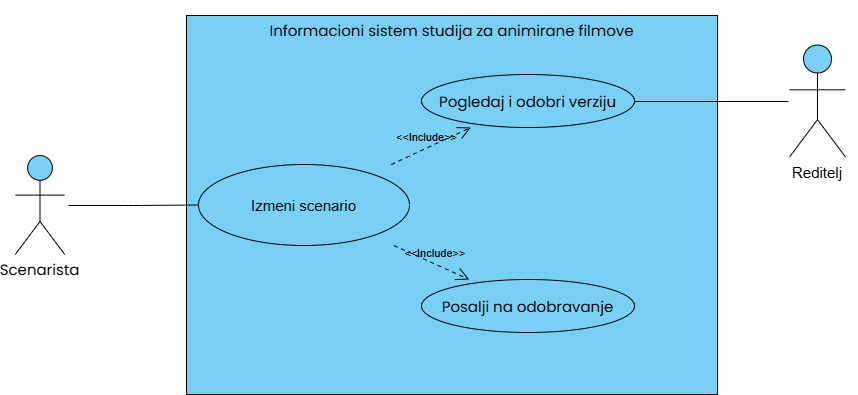
\includegraphics[width=\textwidth]{./dijagrami/dijagrami_slucajeva_upotrebe/izmena_scenarija.png}
	\caption{Dijagram slučaja upotrebe ,,Izmena scenarija''}
 \end{figure}

\begin{figure}[H]
	\centering
	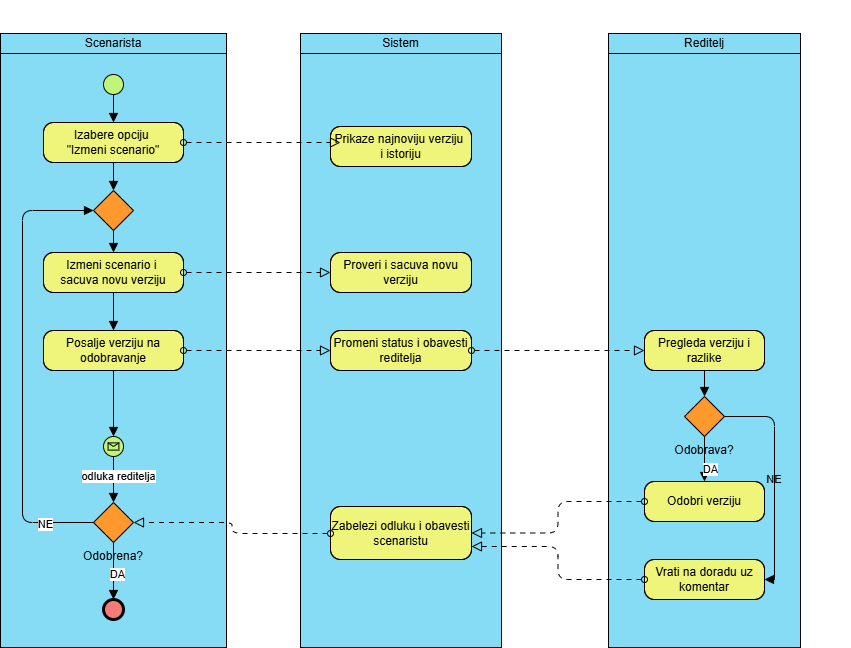
\includegraphics[width=\textwidth]{./dijagrami/bpmn/izmena_scenarija.png}
	\caption{BPMN dijagram ,,Izmena scenarija''}
 \end{figure}

\begin{figure}[H]
	\centering
	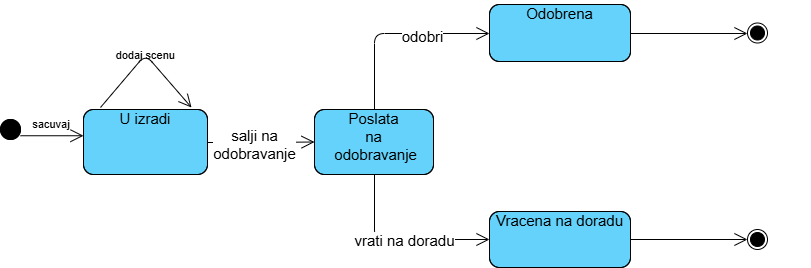
\includegraphics[width=\textwidth]{./dijagrami/dijagrami_stanja/izmena_scenarija.png}
	\caption{Dijagram stanja verzije scenarija}
 \end{figure}

\newpage
